\section{現時点での研究結果}

\begin{frame}
    \begin{center}
        \LARGE 現時点での研究結果
    \end{center}
\end{frame}

\begin{frame}{周期外力付き Rössler 方程式(1/2)}        
    \begin{minipage}{0.4\textwidth}
            \begin{figure}
                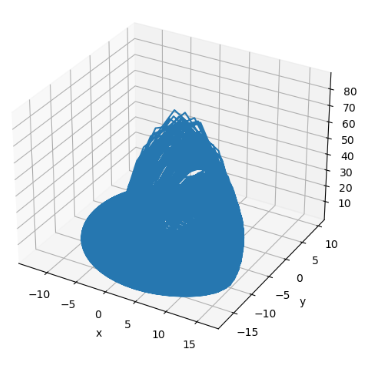
\includegraphics[width=0.7\textwidth]{Fig/Rossler_attractor.png}
                \caption{位相シフトのある周期外力付きのRössler システム}
                \label{rossler_attractor.png} % ラベルを付ける(参照する場合に使用)
            \end{figure}
            \vspace{-.7cm}
            \begin{itemize}
                \item 位相シフト(クロニックジェットラグ)を含む周期外力がある系の予測を Reservoir Computer で行う:
            \end{itemize}
        \end{minipage}
    \begin{minipage}{0.59\textwidth}
        \vspace{-.5cm}
        \begin{align}
            \frac{dx}{dt} &= -y - z + A \sin(t + \Omega(t))\\
            \frac{dy}{dt} &= x + ay \\
            \frac{dz}{dt} &= b + z(x - c)
        \end{align}
        \vspace{-.5cm}
        \begin{itemize}
            \item 外力の振幅$A = 2.0$,変数$a = 0.2,\ b = 0.2,\ c = 5.7$,初期条件$ \left[ x, y, z \right] = [1.0, 1.0, 1.0]$.時間範囲:$[0, 2510]$, 系の周期は $2\pi$ .
            \item $\Omega(t)$ は$t$について定期的に位相シフトを与える関数.ここでは,$4$ 日に一度 $\left[ -12, 12 \right]$ の中からランダムに整数 $n$ をとり $n$ 時間分だけ系を早める(遅らせる)ような $\Omega(t)$ を扱う.    
        \end{itemize}
    \end{minipage}
\end{frame}

\begin{frame}{周期外力付き Rössler 方程式(2/2)}
    \begin{figure}
        %\centering % 画像を中央揃えにする(オプション)
        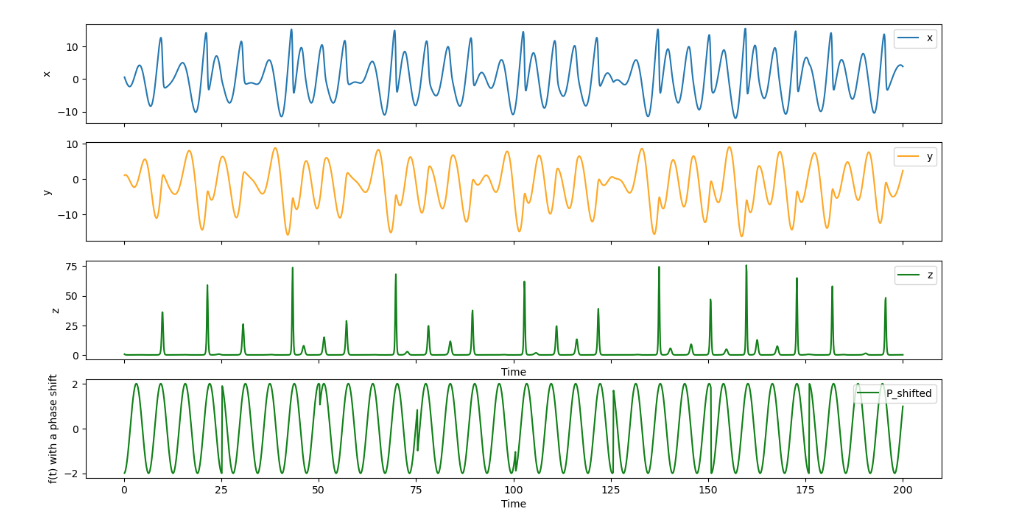
\includegraphics[width=0.75\textwidth]{Fig/Plot_rossler_variables.png}
        \caption{位相シフトのある周期外力付きのRössler システム:\\変数ごとと外力の時系列のグラフ}
        \label{plot_rossler_attractor.png} % ラベルを付ける(参照する場合に使用)
    \end{figure}
\end{frame}

\begin{frame}{Reservoir Computerによる予測:手法}
    $\triangle t = 0.1$ とした.
    \begin{itemize}
        \item Hyperparametersの最適化
        \begin{itemize}
            \item 学習期間: Rössler システムにおける $z$ 変数が観測できないものとして, $x, y$ 変数 と 外力 $f(t)$ を入力する.期間は $\left.\left[ 0, 1000 \right.\right).$ \vspace{.2em}
            \item 損失関数を学習期間全体に対して定義された nrmse として最適化:
            \vspace{.2em}
            \begin{align}
                \text{nrmse}(y, M) = \sqrt{\frac{\sum_{i=0}^{M-1}\left(y_i-\hat{y}_i\right)^2}{M}}
            \end{align}
            \item Hyperparameters は Cell number (N), spectral radius (sr), leaking rate (lr), input scaling (iss), regularization (ridge), random seed(seed). \vspace{.2em}
            \item 最適化アルゴリズムはTPE (Tree-structured Parzen Estimator) algorithm.
        \end{itemize}
        \item Self-evolving 期間
        \begin{itemize}
            \item warming up:
            $\left.\left[ 1000,  1500\right.\right]$, Self-evolving 期間: $\left[ 1500,  2510\right].$
            \item 上のように訓練された Reservoir Computer を用いて,確定的な位相シフトの外力が加わったモデルの時系列データに対しても予測し、平均振幅などの統計量を調べる.
        \end{itemize}
    \end{itemize}
\end{frame}

\begin{frame}{結果}

\end{frame}

\begin{frame}{結果}

\end{frame}

\begin{frame}{結果}

\end{frame}







